\documentclass[12pt]{article}
\usepackage[margin=2.5cm]{geometry}
\usepackage{enumerate}
\usepackage{amsfonts}
\usepackage{amsmath}
\usepackage{fancyhdr}
\usepackage{amsmath}
\usepackage{amssymb}
\usepackage{amsthm}
\usepackage{mdframed}
\usepackage{graphicx}
\usepackage{subcaption}
\usepackage{adjustbox}
\usepackage{listings}
\usepackage{xcolor}
\usepackage{booktabs}
\usepackage[utf]{kotex}
\usepackage{hyperref}

\definecolor{codegreen}{rgb}{0,0.6,0}
\definecolor{codegray}{rgb}{0.5,0.5,0.5}
\definecolor{codepurple}{rgb}{0.58,0,0.82}
\definecolor{backcolour}{rgb}{0.95,0.95,0.92}

\lstdefinestyle{mystyle}{
    backgroundcolor=\color{backcolour},
    commentstyle=\color{codegreen},
    keywordstyle=\color{magenta},
    numberstyle=\tiny\color{codegray},
    stringstyle=\color{codepurple},
    basicstyle=\ttfamily\footnotesize,
    breakatwhitespace=false,
    breaklines=true,
    captionpos=b,
    keepspaces=true,
    numbers=left,
    numbersep=5pt,
    showspaces=false,
    showstringspaces=false,
    showtabs=false,
    tabsize=1
}

\lstset{style=mystyle}

\pagestyle{fancy}
\renewcommand{\headrulewidth}{0.4pt}
\lhead{CSC 373}
\rhead{Worksheet 1 Solution}

\begin{document}
\title{CSC373 Worksheet 1 Solution}
\maketitle

\bigskip

\begin{enumerate}[1.]
    \item

    \begin{lstlisting}
    Strassen_Algorithm(A,B):
        n = A.rows
        let C be a new n x n matrix

        if n == 1
            C_11 = A_11 * B_11

        else partition as in step 3 of strassen's algorithm

            p1 = Strassen_Algorithm(A_11, B_12) -
                 Strassen_Algorithm(A_11, B_22)

            p2 = Strassen_Algorithm(A_11, B_22) +
                 Strassen_Algorithm(A_12, B_22)

            p3 = Strassen_Algorithm(A_21, B_11) +
                 Strassen_Algorithm(A_22, B_11)

            p4 = Strassen_Algorithm(A_22, B_21) -
                 Strassen_Algorithm(A_22, B_11)

            p5 = Strassen_Algorithm(A_11, B_11) +
                 Strassen_Algorithm(A_11, B_22) +
                 Strassen_Algorithm(A_22, B_11) +
                 Strassen_Algorithm(A_22, B_22)

            p6 = Strassen_Algorithm(A_12, B_21) +
                 Strassen_Algorithm(A_12, B_22) -
                 Strassen_Algorithm(A_22, B_21) -
                 Strassen_Algorithm(A_22, B_22)

            p7 = Strassen_Algorithm(A_11, B_11) +
                 Strassen_Algorithm(A_11, B_12) -
                 Strassen_Algorithm(A_21, B_11) -
                 Strassen_Algorithm(A_21, B_12)

            C_11 = p5 + p4 - p2 + p6
            C_12 = p1 + p2
            C_21 = p3 + p4
            C_22 = p5 + p1 - p3 - p7

        return C
    \end{lstlisting}

    \bigskip

    \underline{\textbf{Notes:}}

    \begin{itemize}
        \item Strassen's method for matrix multiplication

        \begin{itemize}
            \item Reduces the time complexity of matrix multiplication from $O(n^3)$ to $O(n^{\log_2 7}) = O(n^{2.81})$

            \item Has four steps

            \bigskip

            \begin{enumerate}[1)]
                \item Divide the input matrics $A$ and $B$ and output matrix $C$
                into $n/2 \times n/2$ submatrices

                \begin{center}
                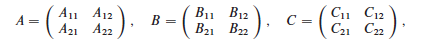
\includegraphics[width=0.7\linewidth]{images/worksheet_1_solution_1.png}
                \end{center}

                \item Create 10 matrices, $S_1, S_2, ..., S_{10}$ each of which is
                $n/2 \times n/2$ and is the sum or difference of two matrices created in step 1

                \bigskip

                $S_1 = B_{12} - B_{22}$

                $S_2 = A_{11} + A_{12}$

                $S_3 = A_{21} + A_{22}$

                $S_4 = B_{21} - B_{11}$

                $S_5 = A_{11} + A_{22}$

                $S_6 = B_{11} + B_{22}$

                $S_7 = A_{12} - A_{22}$

                $S_8 = B_{21} + B_{22}$

                $S_9 = A_{11} - A_{21}$

                $S_{10} = B_{11} + B_{12}$

                \bigskip

                \item Recursively multiply $n/2 \times n/2$ matrices seven times to
                compute the following $n/2 \times n/2$ matrices

                \bigskip

                $P_1 = A_{11} \cdot S_1 = A_{11} \cdot B_{12} - A_{11} \cdot B_{22}$

                $P_2 = S_2 \cdot B_{22} = A_{11} \cdot B_{22} + A_{12} \cdot B_{22}$

                $P_3 = S_3 \cdot B_{11} = A_{21} \cdot B_{11} + A_{22} \cdot B_{11}$

                $P_4 = A_{22} \cdot S_4 = A_{21} \cdot B_{11} + A_{22} \cdot B_{11}$

                $P_5 = S_5 \cdot S_6 = A_{11} \cdot B_{11} + A_{11} \cdot B_{22} + A_{22} \cdot B_{11} + A_{22} \cdot B_{22}$

                $P_6 = S_7 \cdot S_8 = A_{12} \cdot B_{21} + A{12} \cdot B_{22} - A_{22} \cdot B_{21} - A_{22} \cdot B_{22}$

                $P_7 = S_9 \cdot S_{10} = A_{11} \cdot B_{11} + A_{11} \cdot B_{12} - A_{21} \cdot B_{11} - A_{21} \cdot B_{12}$

                \item Construct the four $n/2 \times n/2$ submatrices of the product $C$

                \bigskip

                $C_{11} = P_5 + P_4 - P_2 + P_6 = A_{11} \cdot B_{11} + A_{12} + B_{12}$

                $C_{12} = P_1 + P_2 = A_{11} \cdot B_{12} + A_{12} \cdot B_{22}$

                $C_{21} = P_3 + P_4 = A_21\cdot B_11 + A_{22} \cdot B_{21}$

                $C_{22} = P_5 + P_1 - P_3 - P_7 = A_{22} \cdot B_{22} + A_{21} \cdot B_{12}$

            \end{enumerate}

            \bigskip

            \underline{\textbf{Example:}} Use Strassen's algorithm to compute the matrix product

            \begin{align*}
            \begin{pmatrix}
                1 & 3\\
                7 & 5
            \end{pmatrix}
            \begin{pmatrix}
                6 & 8\\
                4 & 2
            \end{pmatrix}
            \end{align*}

            \begin{itemize}
                \item \textbf{STEP 1}

                \bigskip

                $A_{11} = 1, A_{12} = 3, A_{21} = 7, A_{22} = 5$

                \bigskip

                $B_{11} = 6, B_{12} = 8, B_{21} = 4, B_{22} = 2$

                \bigskip
                \item \textbf{STEP 2}

                \bigskip

                $S_1 = B_{12} - B_{22} = 4 - 2 = 2$

                \bigskip

                $S_2 = A_{11} + A_{12} = 1 + 3 = 4$

                \bigskip

                $S_3 = A_{21} + A_{22} = 7 + 5 = 12$

                \bigskip

                $S_4 = B_{21} - B_{11} = 4 - 6 = -2$

                \bigskip

                $S_5 = A_{11} + A_{22} = 1 + 5 = 6$

                \bigskip

                $S_6 = B_{11} + B_{22} = 6 + 2 = 8$

                \bigskip

                $S_7 = A_{12} - A_{22} = 3 - 5 = -2$

                \bigskip

                $S_8 = B_{21} + B_{22} = 8 + 2 = 10$

                \bigskip

                $S_9 = A_{11} - A_{21} = 3 - 5 = -2$

                \bigskip

                $S_{10} = B_{11} + B_{12} = 6 + 4 = 10$

                \bigskip

                \item \textbf{STEP 3}

                \bigskip

                $P_1 = A_{11} \cdot S_1 = A_{11} \cdot B_{12} - A_{11} \cdot B_{22} = 1 \cdot 4 - 1 \cdot 2 = 2$

                \bigskip

                $P_2 = S_2 \cdot B_{22} = A_{11} \cdot B_{22} + A_{12} \cdot B_{22} = 1 \cdot 2 + 3 \cdot 2 = 8$

                \bigskip

                $P_3 = S_3 \cdot B_{11} = A_{21} \cdot B_{11} + A_{22} \cdot B_{11} = 6 \cdot 7 + 6 \cdot 5 = 72$

                \bigskip

                $P_4 = A_{22} \cdot S_4 = A_{22} \cdot B_{21} - A_{22} \cdot B_{11} = 5 \cdot 4 - 5 \cdot 6 = -10$

                \bigskip

                $P_5 = S_5 \cdot S_6 = A_{11} \cdot B_{11} + A_{11} \cdot B_{22} + A_{22} \cdot B_{11} + A_{22} \cdot B_{22} = 48$

                \bigskip

                $P_6 = S_7 \cdot S_8 = A_{12} \cdot B_{21} + A_{12} \cdot B_{22} - A_{22} \cdot B_{21} - A_{22} \cdot B_{22} = -20$

                \bigskip

                $P_7 = S_9 \cdot S_{10} = A_{11} \cdot B_{11} + A_{11} \cdot B_{12} - A_{21} \cdot B_{11} - A_{21} \cdot B_{12} = -20$

                \bigskip

                \item \textbf{STEP 4}

                \bigskip

                $C_{11} = P_5 + P_4 - P_2 + P_6 = 48 - 10 - 8 - 20 = 10$

                \bigskip

                $C_{12} = P_1 + P_2 = 10$

                \bigskip

                $C_{21} = P_3 + P_4 = 62$

                \bigskip

                $C_{22} = P_5 + P_1 - P_3 - P_7 = 48 + 2 - 72 + 20 = -2$

                \bigskip

            \end{itemize}

            \item Is not preferred in practical purposes

            \bigskip

            \begin{enumerate}[1)]
                \item The constants used in Strassen’s method are high and for a typical application Naive method works better.
                \item For Sparse matrices, there are better methods especially designed for them.
                \item The submatrices in recursion take extra space.
                \item Because of the limited precision of computer arithmetic on noninteger values, larger errors accumulate in Strassen’s algorithm than in Naive Method
            \end{enumerate}
        \end{itemize}

        \bigskip

        \underline{\textbf{References:}}

        \bigskip

        \begin{enumerate}[1)]
            \item GeeksForGeeks, Divide and Conquer | Set 5 (Strassen’s Matrix Multiplication), \href{https://www.geeksforgeeks.org/strassens-matrix-multiplication/}{link}
        \end{enumerate}

        \item Regular matrix multiplication

        \begin{itemize}
            \item
        \end{itemize}

        \item The master method for solving recurrences

        \begin{itemize}
            \item provides 'cookbook' method for solving recurrences
            of the form

            \begin{align*}
                T(n) = aT(n/b) + f(n)
            \end{align*}

            \item depends on the following theorem

            \begin{itemize}
                \item Let $a \leq 1$ and $b > 1$ be constants, let $f(n)$ be a function
                and let $T(n)$ be defined on the nonnegative integers by the recurrence

                \bigskip

                $T(n) = aT(n/b) + f(n)$

                \bigskip

                where we interpret $n/b$ to mean either $\lfloor n/b \rfloor$ or $\lceil n/b \rceil$.
                Then $T(n)$ has the following asymptotic bounds:

                \bigskip

                \begin{enumerate}[1.]
                    \item If $f(n) = O(n^{\log_b a-\epsilon}) for some constant \epsilon > 0, then T(n) = \Theta(n^{\log_b a})$
                    \item If $f(n) = \Theta(n^{\log_b a})$, then $T(n) = \Theta(n^{\log_b a} \lg n)$
                    \item If $f(n) = \Omega(n^{\log_b a + \epsilon})$ for some constant $\epsilon > 0$, and if
                    $af(n/b) \leq cf(n)$ for some constant $c < 1$, and all sufficiently large $n$,
                    then $T(n) = \Theta(f(n))$.
                \end{enumerate}

                \bigskip

                \underline{\textbf{Example:}}

                \bigskip

                $T(n) = 9T(n/3) + n$

                \bigskip

                Here, $a = 9$, $b = 3$, and $f(n) = n = O(n^{\log_3 9 - 1})$ where $\epsilon = 1$.

                \bigskip

                Thus, $T(n) = \Theta(n^{\log_3 9})$ or $T(n) = \Theta(n^2)$


                \bigskip

                \underline{\textbf{Example 2:}}

                \bigskip

                $T(n) = T(2n/3) + 1$

                \bigskip

                Here, $a = 1$, $b = 3/2$, $f(n) = 1 = \Theta(n^{\log_{3/2} 1})$.

                \bigskip

                Thus, $T(n) = \theta(\lg n)$

                \bigskip

                \underline{\textbf{Example 3:}}

                \bigskip

                $T(n) = T(n/4) + n \lg n$

                \bigskip

                Here $a = 1$, $b = 4$, and $f(n) = n \lg n$ has asymptotic lowerbound of $f(n) = \Omega(n^{\log_4 3 + \epsilon}) = \Omega(n)$
                where $\epsilon \approx 0.2$

                \bigskip

                Furthermore,

                \begin{align*}
                    af(n/b) &= (3n/4) \lg n/4\\
                    &= (3/4) n \lg n/4\\
                    &= (3/4) n \lg n/4\\
                    &= 3/4 n\lg n - \lg 4\\
                    &< 3/4 n\lg n\\
                    &= c f(n)
                \end{align*}

                where $c = 3/4$.

                \bigskip

                Thus, $T(n) = \Theta(n\lg n)$

                \bigskip

                \underline{\textbf{Example 4:}}

                \bigskip

            \end{itemize}
        \end{itemize}
    \end{itemize}
\end{enumerate}

\end{document}